%
% management.tex
%
% Copyright (C) 2022 by SpaceLab.
%
% Camera Payload Preliminary Design Review
%
% This work is licensed under the Creative Commons Attribution-ShareAlike 4.0
% International License. To view a copy of this license,
% visit http://creativecommons.org/licenses/by-sa/4.0/.
%

%
% \brief Project management slides.
%
% \author Gabriel Mariano Marcelino <gabriel.mm8@gmail.com>
% \author Vitória Beatriz Bianchin <vitoriabbianchin@gmail.com>
% \author Caique Sales de Miranda Gomes <kiqsmg@gmail.com>
%
% \version 0.1.0
%
% \date 2022/06/24
%


\begin{frame}{Project Management}

    \begin{itemize}
        \item Activities and tasks: GitHub issues/project
        \vspace{0.25cm}
        \item Periodic meetings
        \vspace{0.25cm}
        \item Source files and versioning control: Git/GitHub repository (\href{https://github.com/spacelab-ufsc/adcs}{\textcolor{blue}{https://github.com/spacelab-ufsc/adcs}}) with five development branches:
            \begin{itemize}
                \item \textit{dev\_doc}: Documentation
                \item \textit{dev\_hardware}: Hardware project
                \item \textit{dev\_firmware}: Firmware project
                \item \textit{dev\_mechanical}: Mechanical project
%                \item \textit{dev\_validation}: Validation setup sources
            \end{itemize}
    \end{itemize}

\end{frame}

% #########################################################################
% #########################################################################

\begin{frame}{Product Tree}

    \begin{figure}[!ht]
        \begin{center}
            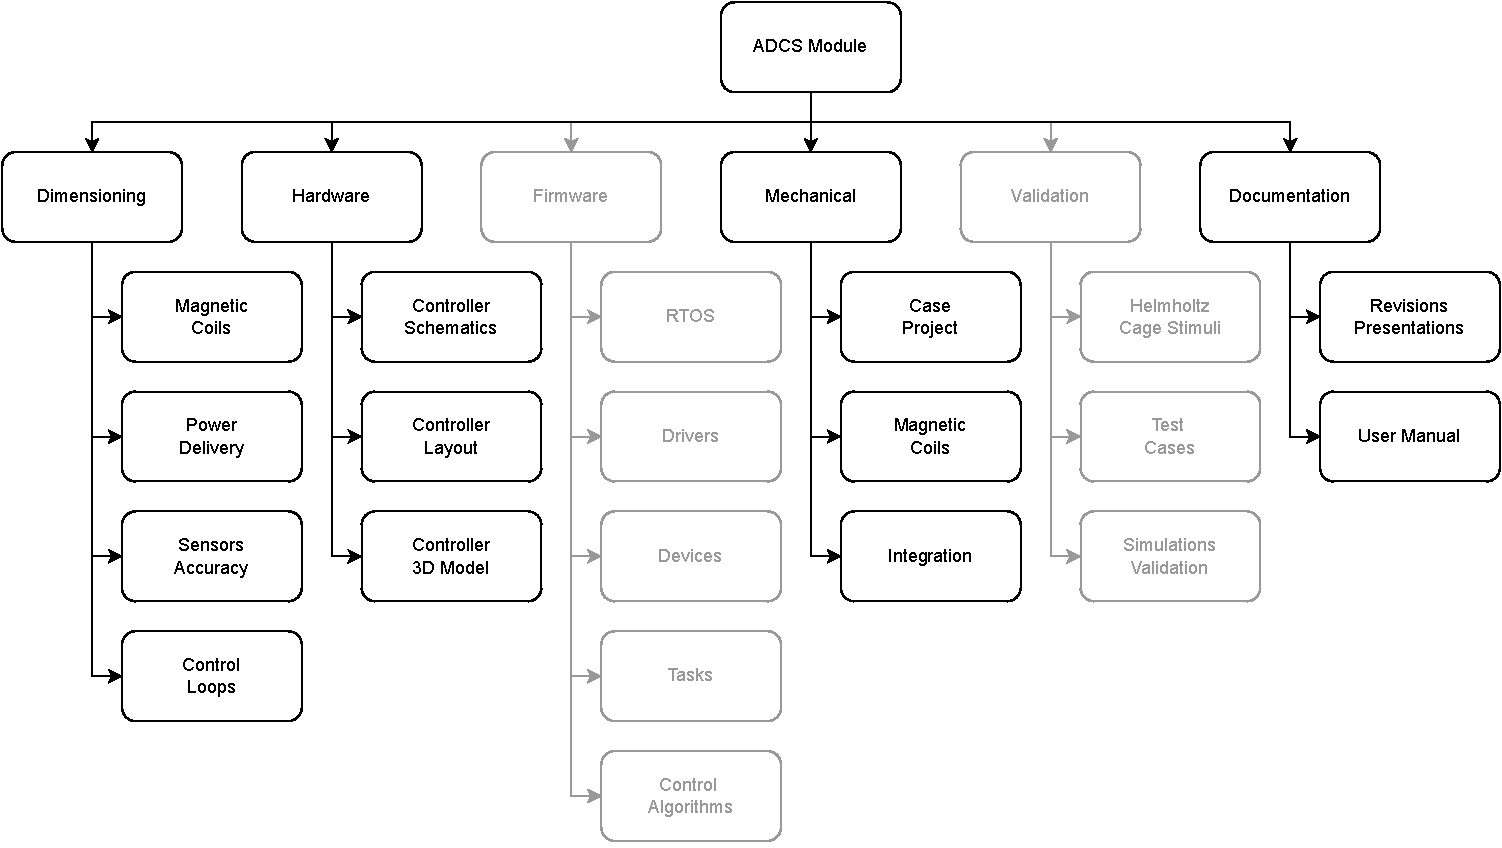
\includegraphics[width=11cm]{figures/product-tree-adcs.pdf}
        \end{center}
    \end{figure}

\end{frame}

% #########################################################################
% #########################################################################

\begin{frame}{Schedule}

\begin{table}[!htb]\tiny
    \centering
    \label{tab:schedule}
    \begin{tabular}{lC{0.15cm}C{0.15cm}C{0.15cm}C{0.15cm}C{0.15cm}C{0.15cm}C{0.15cm}C{0.15cm}C{0.15cm}C{0.15cm}C{0.15cm}C{0.15cm}}
        \toprule[1.5pt]
        \multirow{2}{*}{\textbf{Activity}} & \multicolumn{12}{c}{\textbf{Week}} \\
                          & W1 & W2 & W3 & W4 & W5 & W6 & W7 & W8 & W9 & W10 & W11 & W12 \\
        \midrule                      % 1   2   3   4   5   6   7   8   9   10  11  12
        Project definition            & X &   &   &   &   &   &   &   &   &   &   &     \\
        Bibliographical review        & X &   &   &   &   &   &   &   &   &   &   &     \\
        Project dimensioning          &   & X & X &   &   &   &   &   &   &   &   &     \\
        Component selection           &   & X & X &   &   &   &   &   &   &   &   &     \\
        \textbf{PDR}                  &   &   & \textbf{X} &   &   &   &   &   &   &   &   &     \\
        Mechanical design             &   &   & X & X &   &   &   &   &   &   &   &     \\
        Controller schematics         &   &   & X & X & X &   &   &   &   &   &   &     \\
        Components aquisiton          &   &   &   & X & X & X & X & X &   &   &   &     \\
        Controller PCB layout         &   &   &   & X & X & X & X &   &   &   &   &     \\
        Mockup fabrication            &   &   &   &   &   &   & X &   &   &   &   &     \\
        \textbf{CDR}                  &   &   &   &   &   &   & \textbf{X} &   &   &   &   &     \\
        Controller PCB fabrication    &   &   &   &   &   &   &   & X & X & X & X &     \\
        Case fabrication              &   &   &   &   &   &   &   & X & X &   &   &     \\
        User manual preparation       &   &   &   &   &   &   &   &   & X & X & X &     \\
        Preliminary Electrical tests  &   &   &   &   &   &   &   &   &   &   & X &     \\
        Mechanical integration        &   &   &   &   &   &   &   &   &   &   & X &     \\
        \textbf{AR}                   &   &   &   &   &   &   &   &   &   &   &   & \textbf{X}   \\
        \bottomrule[1.5pt]
    \end{tabular}
\end{table}

{\footnotesize Schedule changes from the original presentation (besides PDR, CDR, and AR):\\5.3:W2, 5.5:W5, 5.7:W9, 5.9:W13}

\end{frame}

% #########################################################################
% #########################################################################

\begin{frame}{Team}

    \begin{table}[!htb]
        \centering
        \label{tab:team}
        \begin{tabular}{ll}
            \toprule[1.5pt]
            \textbf{Role} & \textbf{Name} \\
            \midrule
            \multirow{2}{*}{Management/Support}   & André M. P. de Mattos \\
                                                  & Gabriel M. Marcelino \\
            \midrule
            Dimensioning                          & Matheus Wagner \\
            \midrule
            \multirow{4}{*}{Hardware design}      & Rebecca Q. Do Ó \\
                                                  & Bruno Benedetti \\
                                                  & Caique S. de M. Gomes \\
            \midrule
            Mechanical design                     & Caique S. de M. Gomes \\
            \bottomrule[1.5pt]
        \end{tabular}
    \end{table}

\end{frame}

% #########################################################################
% #########################################################################

\begin{frame}{Cost Estimation\footnote{2 units.}}

\begin{table}[!htb]\scriptsize
    \centering
    \label{tab:cost-estimation}
    \begin{tabular}{lccc}
        \toprule[1.5pt]
        \textbf{Item} & \textbf{Unit (US\$)} & \textbf{Quantity} & \textbf{Total (US\$)} \\
        \midrule
        STM32F103C8T6         & 7.31  & 2  & 14.62 \\
        TCAN330GD             & 3.89  & 2  & 7.78 \\
        Sensors               & 10.00 & 2  & 20.00 \\
        H-Bridge              & 2.00  & 2  & 4.00 \\
        Copper wire           & 10.00 & 1  & 10.00 \\
        Magnetic core         & 10.00 & 4  & 40.00 \\
        Passive components    & 5.00  & 1  & 5.00 \\
        PCB                   & 0.50  & 10 & 5.00 \\
        \midrule
        Total          & \multicolumn{3}{c}{106.40\footnote{Prices in August 2022, without delivery rates or taxes.}} \\
        \bottomrule[1.5pt]
    \end{tabular}
\end{table}

\end{frame}